\documentclass{beamer}
\usepackage[ngerman]{babel}
\usepackage[utf8x]{inputenc}
\usepackage{amsmath,amsfonts,amssymb}
\pdfmapfile{+sansmathaccent.map}
\usetheme{Warsaw}
\usepackage{graphicx}
\begin{document}

\title{Erkennung von Toren beim RoboCup}
\date{2012-07-03}
\author{Elena Noll \and Sven-Hendrik Haase}

\begin{frame}
    \titlepage
\end{frame}

\section*{Gliederung}
\begin{frame}{Gliederung}
    \tableofcontents
\end{frame}

\section{Tore im RoboCup}

\subsection{Middle Size League}
\begin{frame}{Tore im RoboCup}{Middle Size League}
\begin{figure}[htp]
\centering
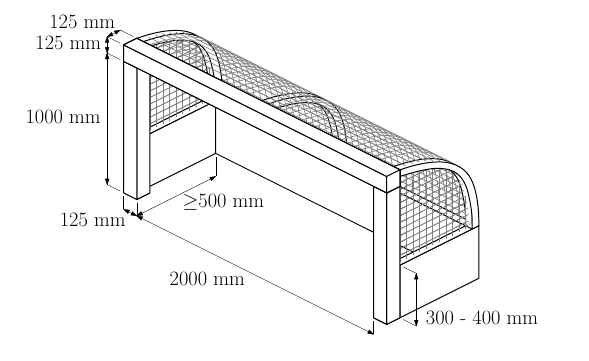
\includegraphics[scale=0.65]{middlesize-goal.png}
\end{figure}
\end{frame}

\subsection{Humanoid League}
\begin{frame}{Tore im RoboCup}{Humanoid League}
\begin{figure}[htp]
\centering
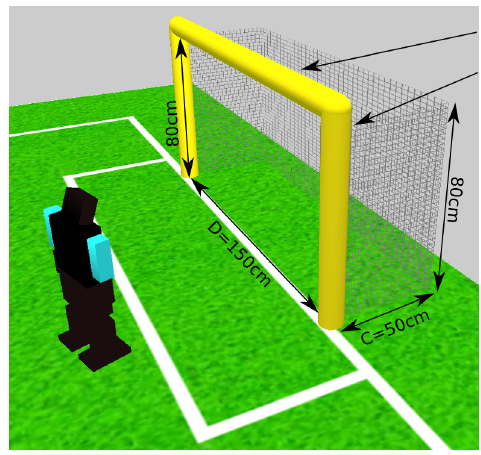
\includegraphics[scale=0.45]{humanoid-kidsize-goal.png}
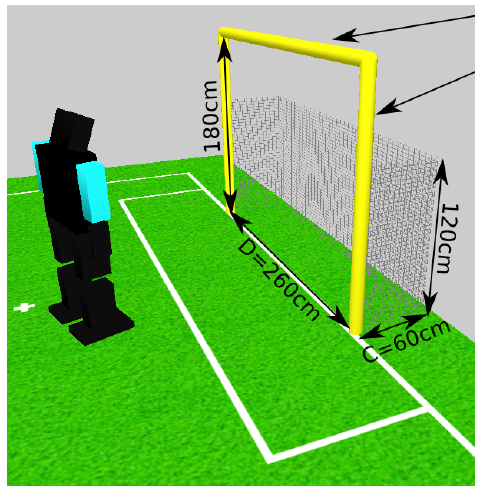
\includegraphics[scale=0.45]{humanoid-adultsize-goal.png}
\end{figure}
\end{frame}

\subsection{Standard Platform League}
\begin{frame}{Tore im RoboCup}{Standard Platform League}
\begin{figure}[htp]
\centering
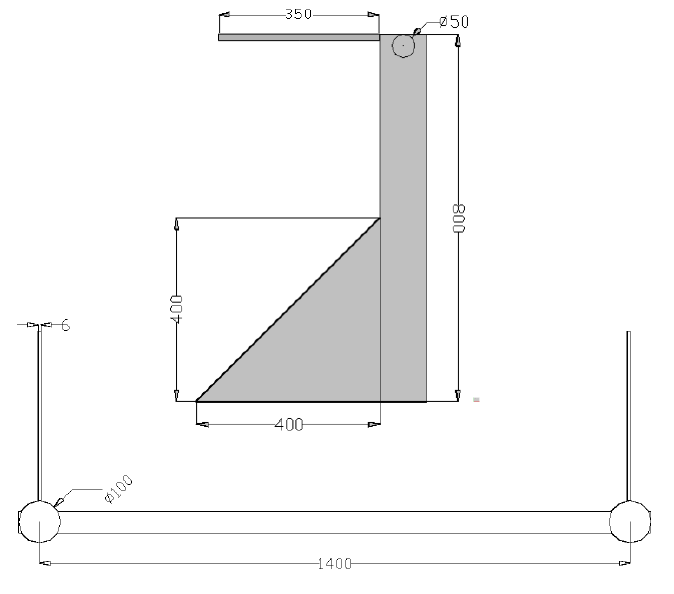
\includegraphics[scale=0.4]{spl-goal.png}
\end{figure}
\end{frame}

\section{Bilderkennung}
\subsection{Probleme}
\begin{frame}{Bilderkennung}{Probleme}
\begin{itemize}
    \item Deformation der Tore je nach Perspektive
    \item Probleme bei Lokalisation durch gleichfarbige Tore
    \item Netze können als Feldlinien erkannt werden
    \item Teile vom Tor können verdeckt sein
    \item Torwart im Tor
\end{itemize}
\end{frame}

\subsection{Erkennung mittels geometrischer Relationen}
\begin{frame}{Bilderkennung}{Erkennung mittels geometrischer Relationen}
\begin{enumerate}
    \item Farbkalibrierung und -segmentierung im YUV-Farbraum
    \item Erkennung des Horizonts
    \item Extraktion der Torpfosten und Modellierung
\end{enumerate}
\end{frame}

\subsubsection{Farbkalibrierung und -segmentierung im YUV-Farbraum}
\begin{frame}{Erkennung mittels geometrischer Relationen}{Farbkalibrierung und -segmentierung im YUV-Farbraum}
\begin{figure}[htp]
\centering
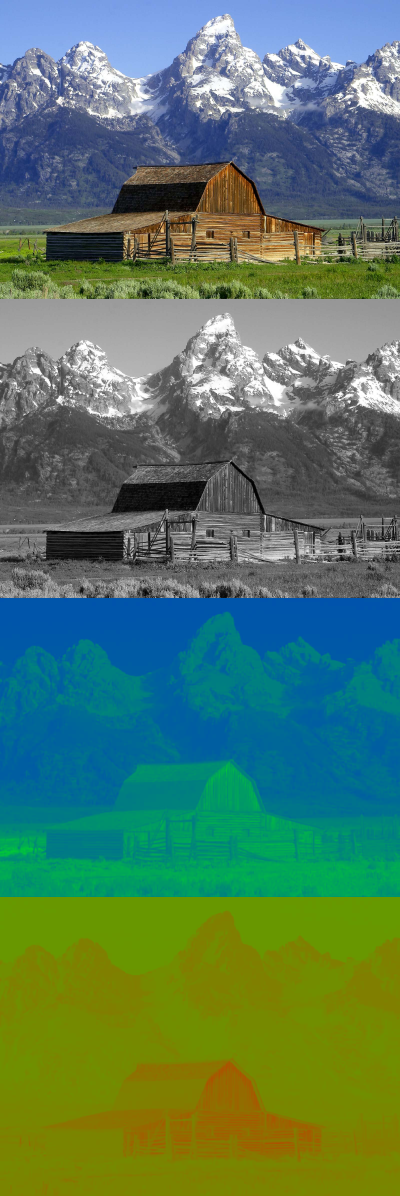
\includegraphics[scale=0.3]{Barn-yuv.png}
\end{figure}
\end{frame}

\begin{frame}{Erkennung mittels geometrischer Relationen}{Farbkalibrierung und -segmentierung im YUV-Farbraum}
\begin{figure}[htp]
\centering
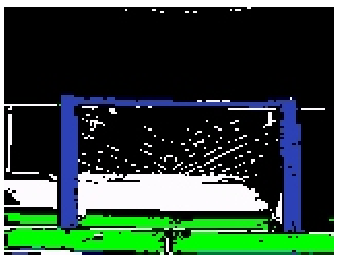
\includegraphics[scale=0.9]{segmented-view2.png}
\end{figure}
\end{frame}

\begin{frame}{Erkennung mittels geometrischer Relationen}{Farbkalibrierung und -segmentierung im YUV-Farbraum}
\begin{figure}[htp]
\centering
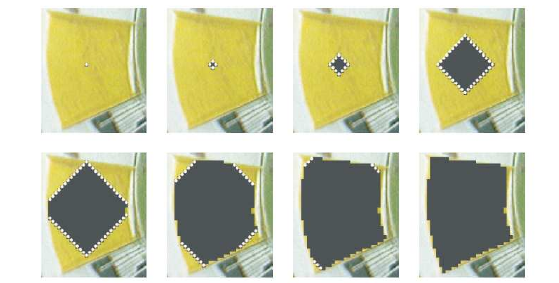
\includegraphics[scale=0.7]{region-growing.png}
\end{figure}
\end{frame}

\begin{frame}{Erkennung mittels geometrischer Relationen}{Farbkalibrierung und -segmentierung im YUV-Farbraum}
\begin{figure}[htp]
\centering
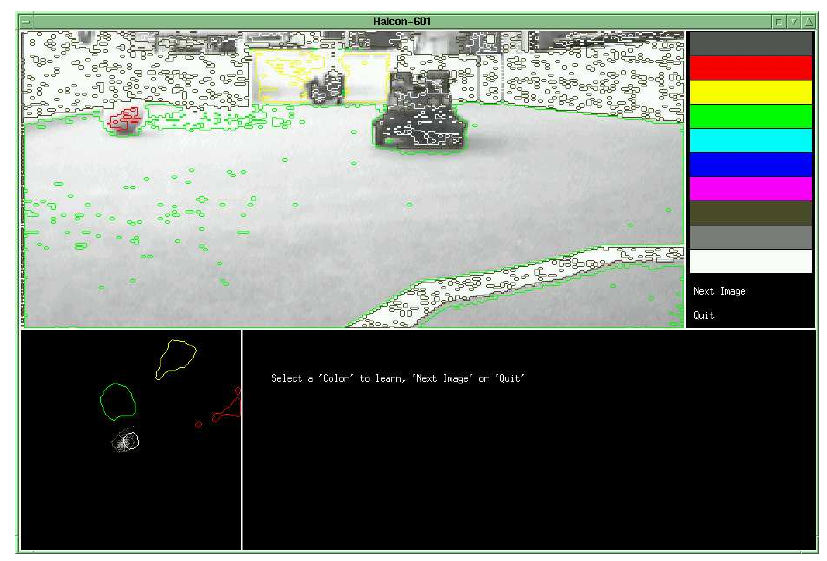
\includegraphics[scale=0.4]{training-tool.png}
\end{figure}
\end{frame}

\begin{frame}{Erkennung mittels geometrischer Relationen}{Farbkalibrierung und -segmentierung im YUV-Farbraum}
\begin{figure}[htp]
\centering
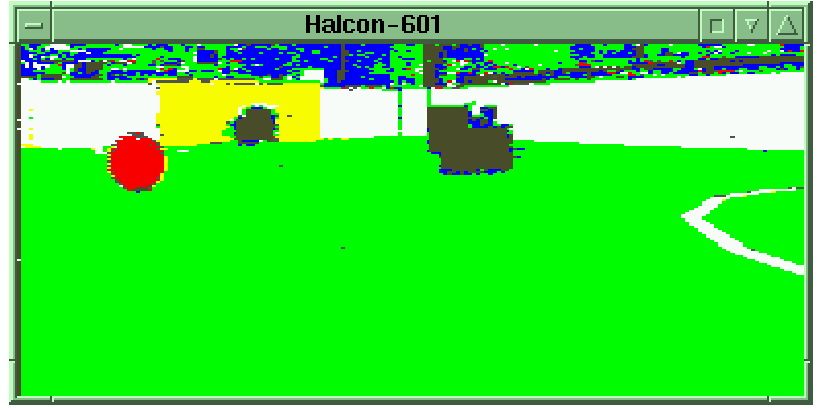
\includegraphics[scale=0.5]{segmented-view.png}
\end{figure}
\end{frame}

\subsubsection{Erkennung des Horizonts}
\begin{frame}{Erkennung mittels geometrischer Relationen}{Erkennung des Horizonts}
\begin{figure}[htp]
\centering
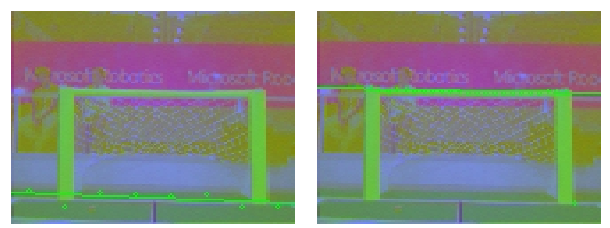
\includegraphics[scale=0.6]{geometric-plane.png}
\end{figure}
\end{frame}

\subsubsection{Extraktion der Torpfosten und Modellierung}
\begin{frame}{Erkennung mittels geometrischer Relationen}{Extraktion der Torpfosten und Modellierung}
\begin{figure}[htp]
\centering
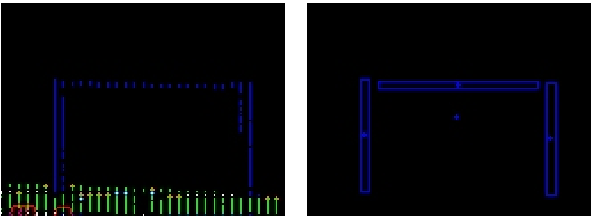
\includegraphics[scale=0.6]{goal-blobs.png}
\end{figure}
\end{frame}

\subsubsection{Beispiele}
\begin{frame}{Erkennung mittels geometrischer Relationen}{Beispiele}
\begin{figure}[htp]
\centering
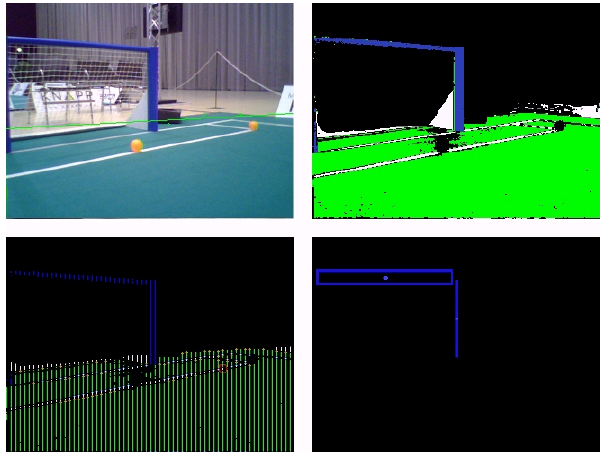
\includegraphics[scale=0.45]{example-detection1.png}
\end{figure}
\end{frame}

\begin{frame}{Erkennung mittels geometrischer Relationen}{Beispiele}
\begin{figure}[htp]
\centering
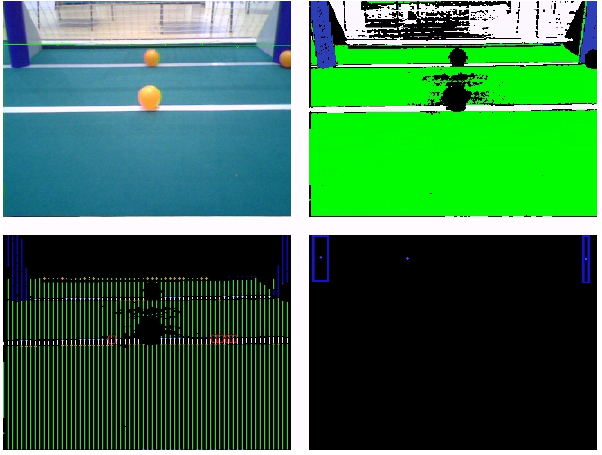
\includegraphics[scale=0.5]{example-detection2.png}
\end{figure}
\end{frame}

\begin{frame}{Erkennung mittels geometrischer Relationen}{Beispiele}
\begin{figure}[htp]
\centering
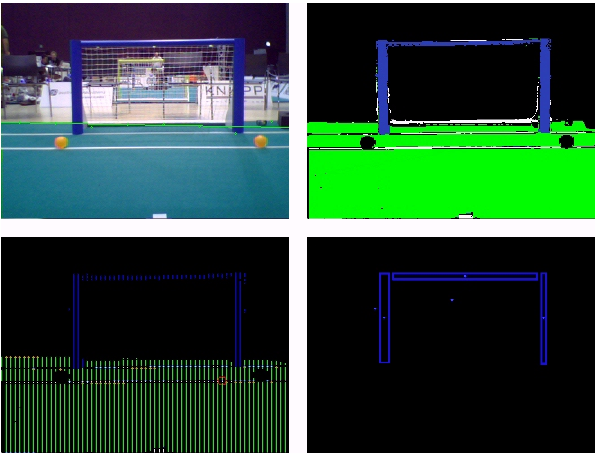
\includegraphics[scale=0.5]{example-detection3.png}
\end{figure}
\end{frame}

\begin{frame}{Erkennung mittels geometrischer Relationen}{Beispiele}
\begin{figure}[htp]
\centering
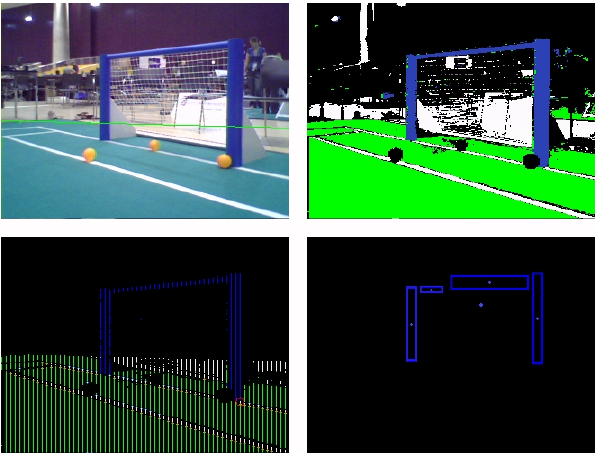
\includegraphics[scale=0.5]{example-detection4.png}
\end{figure}
\end{frame}

\subsection{Erkennung mittels Hough-Transformation}
\begin{frame}{Bilderkennung}{Erkennung mittels Hough-Transformation}
\begin{enumerate}
    \item Farbfilterung im HSV-Farbraum
    \item Eckenfilter für Torkonturen
    \item Hough-Transformation erkennt Torsegmente
    \item Aufspannung des Tormodells durch Eckpunkte
\end{enumerate}
\end{frame}

\subsubsection{Farbfilterung im HSV-Farbraum}
\begin{frame}{Erkennung mittels Hough-Transformation}{Farbfilterung im HSV-Farbraum}
\begin{figure}[htp]
\centering
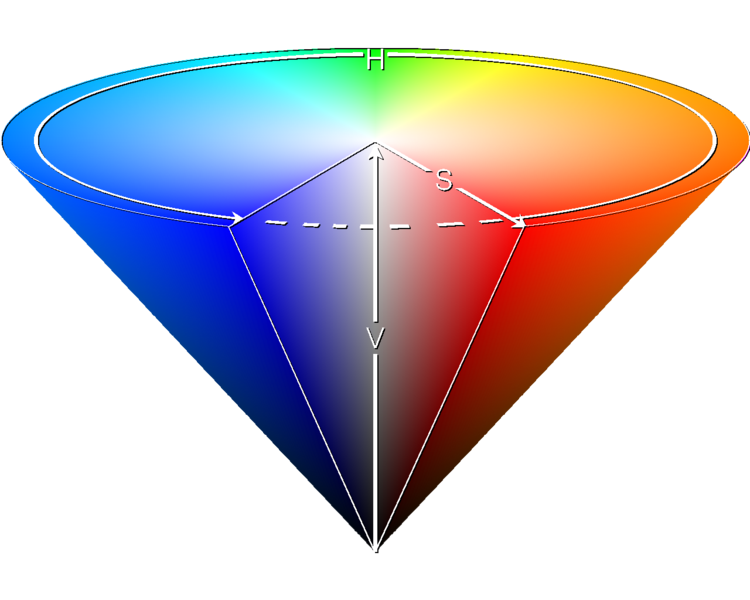
\includegraphics[scale=0.3]{750px-HSV_cone.png}
\end{figure}
\end{frame}

\subsubsection{Zielsetzung der Hough-Transformation}
\begin{frame}{Bilderkennung}{Zielsetzung der Hough-Transformation}
\begin{itemize}
    \item Finden von vorgegebenen geometrischen Strukturen in einem (segmentierten) Bild
    \item Überprüft wird, ob einzelne Segmente der Referenzstruktur ähnlich sind
\end{itemize}
\end{frame}

\subsubsection{Beispiel}
\begin{frame}[label=hough]{Erkennung mittels Hough-Transformation}{Beispiel}
\begin{figure}[htp]
\centering
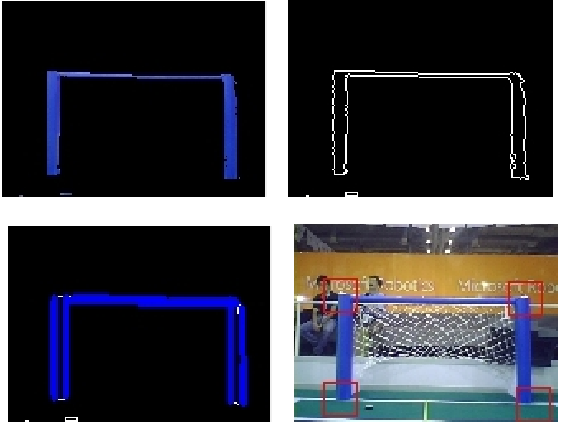
\includegraphics[scale=0.5]{hough-transformation-method.png}
\end{figure}
\end{frame}

\begin{frame}{Erkennung mittels Hough-Transformation}{Beispiel}
    \begin{figure}[htbp]
	\centering
	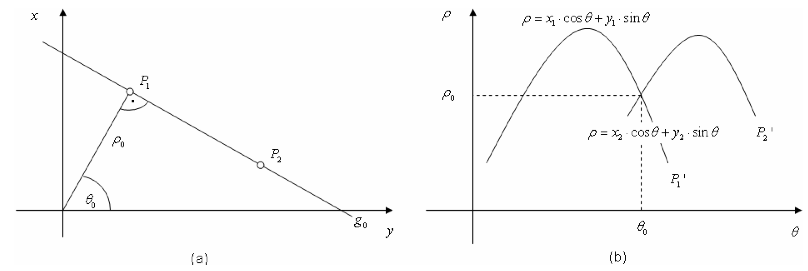
\includegraphics[scale=0.4]{hough-transformation.png}
	\end{figure}
	 \href{http://www.activovision.com/octavi/doku.php?id=hough_transform}{Applet}
\end{frame}

\againframe{hough}

\subsubsection{Eigenschaften der Hough-Transformation}
\begin{frame}{Bilderkennung}{Eigenschaften der Hough-Transformation}
\begin{itemize}
    \item Robust gegenüber Rauschen und systematischen Fehlern
    \item Erkennt auch teilweise verdeckte (unvollständige) Strukturen
\end{itemize}
\end{frame}

\section*{Fragen}
\begin{frame}{Fragen}
Noch Fragen?
\end{frame}

\section*{Quellenverzeichnis}
\begin{frame}{Quellenverzeichnis}
\begin{tiny}
\begin{itemize}
    \item Official RoboCup Standard Platform League Rules for 2010/2011/2012  (http://wiki.robocup.org/wiki/Standard\_Platform\_League\#Rules)
    \item Official RoboCup Humanoid League Rules for 2009/2010/2011/2012 (http://wiki.robocup.org/wiki/Humanoid\_League\#Rules)
    \item Official RoboCup Middle Size League Rules for 2009/2010/2011/2012 (http://wiki.robocup.org/wiki/Middle\_Size\_League\#Rules)
    \item Fast Image Segmentation, Object Recognition and Localization in a RoboCup Scenario (http://citeseerx.ist.psu.edu/viewdoc/download?doi=10.1.1.27.1388\&rep=rep1\&type=pdf)
    \item Recognition of Standard Platform RoboCup Goals (http://gsyc.es/jmplaza/papers/jopha-2010.pdf)
    \item YUV-Farbmodell (http://de.wikipedia.org/wiki/YUV-Farbmodell)
    \item RGB-Farbraum (http://de.wikipedia.org/wiki/RGB-Farbraum)
    \item HSV-Farbraum (http://de.wikipedia.org/wiki/HSV-Farbraum)
    \item k-Means-Algorithmus (http://de.wikipedia.org/wiki/K-Means-Algorithmus)
    \item Die Hough-Transformation (http://page.mi.fu-berlin.de/alt/vorlesungen/sem04/10\_6Die\%20Hough.doc)
\end{itemize}
\end{tiny}
\end{frame}

\end{document}